\documentclass{standalone}
\usepackage{tikz}

\begin{document}
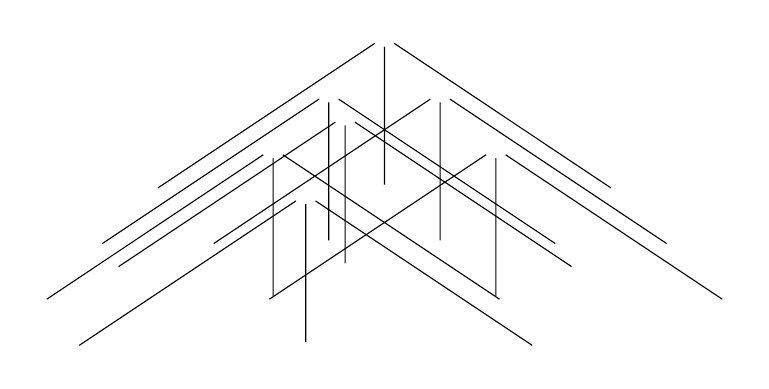
\begin{tikzpicture}[level distance=2cm,
    level 1/.style={sibling distance=3cm},
    level 2/.style={sibling distance=2cm},
    level 3/.style={sibling distance=1cm}]
    
    % Base level (3 nodes)
    \node (base) {}
        child { node (base1) {} }
        child { node (base2) {} }
        child { node (base3) {} };
        
    % Middle level (3 nodes)
    \node (middle1) [below left of=base] {}
        child { node (middle1a) {} }
        child { node (middle1b) {} }
        child { node (middle1c) {} };
        
    \node (middle2) [below right of=base] {}
        child { node (middle2a) {} }
        child { node (middle2b) {} }
        child { node (middle2c) {} };
        
    \node (middle3) [below of=base, xshift=-0.5cm] {}
        child { node (middle3a) {} }
        child { node (middle3b) {} }
        child { node (middle3c) {} };
        
    % Top level (3 nodes)
    \node (top1) [below left of=middle1] {}
        child { node (top1a) {} }
        child { node (top1b) {} }
        child { node (top1c) {} };
        
    \node (top2) [below right of=middle2] {}
        child { node (top2a) {} }
        child { node (top2b) {} }
        child { node (top2c) {} };
        
    \node (top3) [below of=middle3, xshift=-0.5cm] {}
        child { node (top3a) {} }
        child { node (top3b) {} }
        child { node (top3c) {} };
        
\end{tikzpicture}
\end{document}